\chapter{Results}
\label{cha:results}

\section{GBFV-PIRANA versus one-hot encoding}

\subsection{Communication cost}
One-hot encoding can be used to reduce the communication cost when querying one element from a database.
The communication cost in PIRANA when querying one element is $m$ ciphertexts, where $m$ is equal to $O\!\left(\sqrt[k]{k! \, n}  + k \right)$. The communication cost in one-hot encoding is equal to one ciphertext for the rows, because there are as many rows as slots, and $t / s$ ciphertexts for the columns, since there are more columns than slots in a ciphertext. So the query communication cost, which is the amount of ciphertexts sent from client to server, is equal to:  
\begin{equation}
    \texttt{query communication cost} = 1 + \frac{n}{s^2}
\end{equation}

As can be deduced from the formulas above, the communication cost in one-hot encoding will be lower for small databases (small $n$). In Table \ref{tab:query_PIRANA_OH} the number of elements is shown from which on PIRANA has a lower query communication cost (number of ciphertexts that constitute the query) than one-hot encoding. The results are shown for different amount of slots $s$ and a Hamming weight of $k=2$.

\begin{figure}[h]
    \centering
    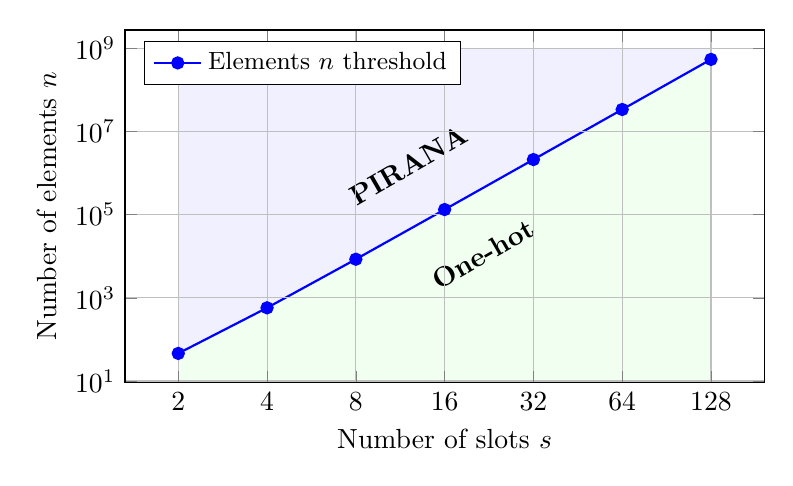
\begin{tikzpicture}
        \begin{semilogxaxis}[
            xlabel={Number of slots $s$},
            ylabel={Number of elements $n$},
            xmode=log,
            ymode=log,
            log basis x={2},
            log basis y={10},
            grid=major,
            width=0.8\textwidth,
            height=0.5\textwidth,
            legend pos=north west,
            legend style={font=\small},
            xtick={2,4,8,16,32,64,128},
            xticklabels={2,4,8,16,32,64,128},
            axis on top,
        ]
        % Fill region above line (GBFV better)
        \fill[blue!20, opacity=0.3] 
            (axis cs:2,46) -- (axis cs:4,574) -- (axis cs:8,8446) -- 
            (axis cs:16,132094) -- (axis cs:32,2101246) -- 
            (axis cs:64,33570814) -- (axis cs:128,536936446) --
            (axis cs:128,1e9) -- (axis cs:2,1e9) -- cycle;
        
        % Fill region below line (One-Hot better)
        \fill[green!20, opacity=0.3] 
            (axis cs:2,10) -- (axis cs:128,10) -- 
            (axis cs:128,536936446) -- (axis cs:64,33570814) --
            (axis cs:32,2101246) -- (axis cs:16,132094) -- 
            (axis cs:8,8446) -- (axis cs:4,574) -- (axis cs:2,46) -- cycle;
        
        \addplot[blue, mark=*, thick] coordinates {
            (2, 46)
            (4, 574)
            (8, 8446)
            (16, 132094)
            (32, 2101246)
            (64, 33570814)
            (128, 536936446)
        };
        \addlegendentry{Elements $n$ threshold}
        
        % Add labels above and below the line 
        \node[above=10pt, rotate=30, font=\bfseries] at (axis cs:13,132094) {PIRANA};
        \node[below=10pt, rotate=30, font=\bfseries] at (axis cs:20,132094) {One-hot};
        \end{semilogxaxis}
    \end{tikzpicture}
    \caption{Number of elements $n$ from when PIRANA has less communication cost than one-hot encoding (results are indicated for different amount of slots $s$ and Hamming weight $k=2$).}
    \label{tab:query_PIRANA_OH}
\end{figure}

\subsection{Performance}
In this section, one-hot encoding and PIRANA are compared, both implemented with a GBFV scheme. 
To compare both protocols with each other, the same GBFV scheme is implemented. The scheme will use $N=2^6$ and $N=2^8$ as degree of the cyclotomic polynomial ring for respective plaintext moduli of $~32 bits$ and $~64 bits$. One element will be randomly selected from the database. Both schemes are compared for speed of query generation, server response time and decryption and recomposition time. The comparison is done for multiple databases, containing a number of elements varying from $2^8$ to $2^{13}$. The element size is 1024 bits. The respective times are shown in Table \ref{tab:OH_PIRANA_comparison_p32} and \ref{tab:OH_PIRANA_comparison_p64}.

%Pirana vs one-hot table
\begin{table}[t]
    \centering
    \caption{Performance comparison of one-hot encoding and GBFV-PIRANA for plaintext modulus $\sim32$ bits}
    \label{tab:OH_PIRANA_comparison_p32}
    \resizebox{\textwidth}{!}{%
    \begin{tabular}{l l cccccc}
        \toprule
        & \# elements $n$ 
        & $2^8$ & $2^9$ & $2^{10}$ & $2^{11}$ & $2^{12}$ & $2^{13}$\\
        & DB Size (KB) & 32 & 64 & 128 & 256 & 512 & 1024\\
        \midrule
        \multirow{3}{*}{\begin{tabular}[c]{@{}l@{}}PIRANA\end{tabular}}
        & Query generation (s) & 0.010 & 0.011 & 0.014 & 0.019 & 0.026 & 0.038\\
        & Server response (s) & 0.0356 & 0.0818 & 0.1689 & 0.3560 & 0.7409 & 1.5703 \\
        & Dec. and recomposition (s) & 0.006 & 0.006 & 0.006 & 0.007 & 0.007 & 0.008 \\
        \midrule
        \multirow{3}{*}{\begin{tabular}[c]{@{}l@{}}One-hot\end{tabular}}
        & Query generation (s) & 0.006 & 0.007 & 0.008 & 0.011 & 0.016 & 0.027 \\
        & Server response (s) & 0.0705 & 0.1206 & 0.2259 & 0.4643 & 1.0582 & 2.7632 \\
        & Dec. and recomposition (s) & 0.005 & 0.005 & 0.005 & 0.005 & 0.005 & 0.005\\
        \bottomrule
    \end{tabular}
    }
\end{table}

\begin{table}[t]
    \centering
    \caption{Performance comparison of one-hot encoding and GBFV-PIRANA for plaintext modulus $\sim64$ bits}
    \label{tab:OH_PIRANA_comparison_p64}
    \resizebox{\textwidth}{!}{%
    \begin{tabular}{l l cccccc}
        \toprule
        & \# elements $n$ 
        & $2^8$ & $2^9$ & $2^{10}$ & $2^{11}$ & $2^{12}$ & $2^{13}$\\
        & DB Size (KB) & 32 & 64 & 128 & 256 & 512 & 1024\\
        \midrule
        \multirow{3}{*}{\begin{tabular}[c]{@{}l@{}}PIRANA\end{tabular}}
        & Query generation (s) & 0.067 & 0.080 & 0.102 & 0.136 & 0.186 & 0.251 \\
        & Server response (s) & 0.4431 & 0.9560 & 1.9430 & 4.4696 & 10.5309 & 26.1016\\
        & Dec. and recomposition (s) & 0.028 & 0.028 & 0.029 & 0.031 & 0.033 & 0.036\\
        \midrule
        \multirow{3}{*}{\begin{tabular}[c]{@{}l@{}}One-hot\end{tabular}}
        & Query generation (s) & 0.052 & 0.068 & 0.101 & 0.166 & 0.300 & 0.536 \\
        & Server response (s) & 0.2196 & 0.4619 & 1.1564 & 3.2916 & 10.7572 & 38.2325\\
        & Dec. and recomposition (s) & 0.028 & 0.028 & 0.028 & 0.028 & 0.028 & 0.028 \\
        \bottomrule
    \end{tabular}
    }
\end{table}

\subsection{Database processing time}
Before doing any measurements, the database has to be created and processed. The database creation time is the time it takes to create the database of big integers. The database processing time is the time it takes to preprocess the database for querying. For GBFV-PIRANA, preprocessing the databases consists of converting every column of the database into a slotted plaintext, that can later be used for a ciphertext-plaintext multiplication. On the other hand, for one-hot encoding, preprocessing the database consists of setting every chunk of the big integer database into a DenseMatrixMul, which is a type of plaintext matrix that can later be used for a matrix-vector multiplication with ciphertexts.

Note that for one-hot encoding, the server will perform a matrix-vector multiplication. To do this multiplication, a circuit is created, which is evaluated to perform the multiplication. A downside of this approach is that the circuit has to be created for every chunk of a database. This leads to huge server response time when calling this multiplication for a first time. Once the circuit is created, evaluating the circuit becomes faster, since the circuit was already created. This is not a step of the database processing, but it is still a set-up time that has to be taken into account.

The database processing times (including the server response time) for one-hot encoding and GBFV-PIRANA, for different database sizes and different plaintext moduli (so different amount of slots), are shown in Table \ref{tab:db_processing_time}. 

\begin{table}[t]
    \centering
    \caption{Database processing times for one-hot and GBFV-PIRANA, for $N=2^8$}
    \label{tab:db_processing_time}
    \resizebox{0.85\textwidth}{!}{%
    \begin{tabular}{l cccccc}
        \toprule
        Database size $n$ & 
        $2^8$ & $2^9$ & $2^{10}$ & $2^{11}$ & $2^{12}$ & $2^{13}$\\
        \midrule
        GBFV-PIRANA (m) & 0.285 & 0.571 & 1.146 & 2.326 & 4.890 & 10.533 \\
        One-hot (s) & 0.001 & 0.001 & 0.002 & 0.004 & 0.009 & 0.019\\
        \bottomrule
    \end{tabular}
    }
\end{table}


\section{GBFV-PIRANA - parameter optimization}
\label{sec:GBFVPIRbest}
To find the optimal parameters for a GBFV-PIRANA implementation, $N$ is set to $2^8$, the number of elements is set to $2^{12}$ and the size of one element is 512-bit. The amount of slots will be determined by the plaintext modulus. This section compares slots with plaintext modulus going from $16$-bit up to $2048$-bit. Query generation time, server response time and decryption and recomposition times are shown in Table \ref{tab:GBFV_PIRANA_plaintext}. 

\begin{table}[t]
    \centering
    \caption{Performance comparison of GBFV-PIRANA with different plaintext moduli ($N^8$, $512$-bits element size, $2^{12}$ elements)}
    \label{tab:GBFV_PIRANA_plaintext}
    \resizebox{\textwidth}{!}{%
    \begin{tabular}{l cccccccc}
        \toprule
        plaintext modulus (bits) & $2^4$ & $2^5$ & $2^6$ & $2^7$ & $2^8$ & $2^9$ & $2^{10}$ & $2^{11}$\\
        number of slots $s$ & 16 & 64 & 8 & 32 & 16 & 8 & 4 & 2 \\
        \midrule
        Query generation (s) & 0.136 & 0.108 & 0.229 & 0.155 & 0.216 & 0.398 & 1.140 & 2.758 \\
        Server response (s) & 3.0285 & 0.2676 & 6.0063 & 0.2630 & 2.0646 & 1.5483 & 1.3357 & 2.2908 \\
        Dec. and recomposition (s) & 0.021 & 0.041 & 0.027 & 0.037 & 0.058 & 0.073 & 0.071 & 0.090 \\
        \bottomrule
    \end{tabular}
    }
\end{table}

\section{GBFV-PIRANA versus BFV-PIRANA}

The PIRANA-paper by Liu et al. describes a PIR protocol based on BFV. In this thesis, the same protocol is implemented but using a GBFV scheme. This section compares the performance of both implementations. The performance results for the BFV-PIRANA were already shown in Table \ref{tab:pir_comparison}. The GBFV implementation of PIRANA uses $N=2^{13}$, has a payload size of 20 KB (as in the PIRANA-paper). The plaintext modulus size is set to 128 bits, hereby creating 1024 slots. The plaintext modulus size is chosen based on the results of the previous section, where using this plaintext modulus showed lower query generation, server response and decryption and recomposition times. 

\begin{table}[t]
    \centering
    \caption{Performance of GBFV-PIRANA, when using $N=2^{13}$ and payload size 20 KB)}
    \label{tab:GBFV_BFV-PIRANA_comparison}
    \resizebox{0.75\textwidth}{!}{%
    \begin{tabular}{l ccccc}
        \toprule
        \# elements $n$ 
        $2^8$ & $2^9$ & $2^{10}$ & $2^{11}$ & $2^{12}$\\
        DB Size (KB) & 32 & 64 & 128 & 256 \\
        \midrule
        Query generation (s) & 15.988 & 15.583 & 15.280 & 15.986\\
        Server response (s) & 13.6678 & 13.5988 & 13.5965 & 22.8538\\
        Dec. and recomposition (s) & 56.418 & 56.548 & 56.349 & 63.738 \\
        \bottomrule
    \end{tabular}
    }
\end{table}

The implementation of BFV-PIRANA is limited: the maximum plaintext modulus has size 32 bits, and the implementation is only available for small elements (where the element size is smaller than the plaintext size).

Two comparisons are performed for plaintext sizes of 16 and 32 bits with \( N = 2^{10} \). For GBFV, the polynomials \( t(x) \) are chosen as \( t(x) = X^{2^8} - 2 \) and \( t(x) = X^{2^6} - 288 \), thus creating 256 and 64 slots for the 16- and 32-bit cases, respectively. The same database is used for both comparisons, with 1024 elements of size 16 or 32 bits, depending on the plaintext modulus. The results of the performance comparison of these two implementations are shown in Table~2.

\begin{table}[t]
    \centering
    \caption{Performance of GBFV-PIRANA and BFV-PIRANA, when using $N=2^{10}$ and payload size 1024bits)}
    \label{tab:GBFV_BFV-PIRANA_comparison_fheanor}
    \resizebox{\textwidth}{!}{%
    \begin{tabular}{l cccc}
        \toprule
         & Query generation (s) & Server response (s) & Decryption (s) & Total (s) \\
        \midrule
        GBFV ($p=16$) (s) & 0.505 & 0.107 & 0.086 & 0.698 \\
        BFV ($p=16$) (s) & 0.012 & 0.006 & 0.105 & 0.124\\
        \midrule
        GBFV ($p=32$) (s) & 0.530 & 0.028 & 0.445 & 1.003\\
        BFV ($p=32$) (s) & - & - & - & -\\
        \midrule 
        Speedup ($p=16$) & 41.83x & 18.42 & 0.82x & 5.65x \\
        \bottomrule
    \end{tabular}
    }
\end{table}

% \section{Overhead large versus small payload}
% Two GBFV-PIRANA protocols are implemented in the code of this thesis. The first protocol can only take small payloads, where the payload is smaller than the plaintext modulus. The second protocol allows for handling large playloads, larger than the plaintext modulus. Here these two implementations are compared in terms of performance (query generation time, server response time and decryption and recomposition time). 
% % The difference in performance between small and large payload GBFV-PIRANA is overhead caused by the implementation of large payloads. When taking small elements, some functions are still evaluated while there is no need to (e.g. finding in how many chunkgs a payload needs to be split).


